\documentclass[utf8]{article}

\usepackage[utf8]{inputenc}

\usepackage[parfill]{parskip}

\usepackage{amsmath}
\usepackage{amssymb}
\usepackage{amsfonts}
\usepackage{graphicx}
\usepackage{float}
\usepackage{fullpage}
\usepackage{hyperref}
\usepackage{fancyvrb}
\usepackage[dvipsnames]{xcolor}
%------------------------------------------------------------------------------

\title{Software Requirements Document: \\ Quorridor}
\author{MERIAN Emile, ABRAHAM Théo, VINOVRSKI Alexandre, DIMITROV Mark,\\ CHICA COBO Sofia,
HORII Hisao, LEDUC Camille, BOLLENGIER Thomas}

\date{23 Novembre 2021}

\begin{document}
\maketitle

\begin{figure}[H]
  \centering
  
\includegraphics[scale=0.4]{img/logo.png}
\end{figure}

\newpage
\tableofcontents

\newpage

%------------------------------------------------------------------------------
\section{Introduction}
  \subsection{But du projet}
  \subsection{Glossaire}
  \subsection{Historique}


\section{Besoins utilisateur: Fonctionnels}

\begin{figure}[H]
  \centering
  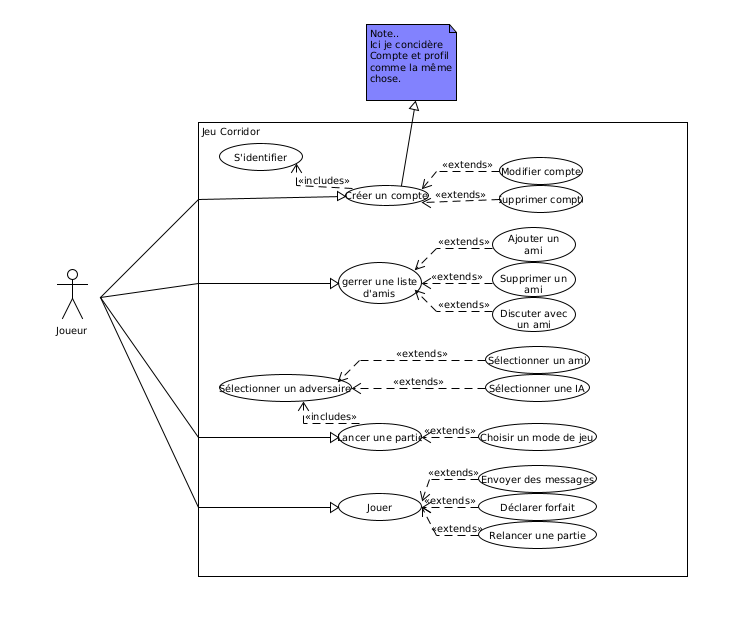
\includegraphics[scale=0.6]{img/ClientUseCase.png}
\end{figure}

  \subsection{Connexion/Création de compte}
    \subsubsection{Inviter un ami}
  \subsection{Chat}
  \subsection{Menu}
    \subsubsection{Créer une partie}
    \subsubsection{Rejoindre une partie}
    \subsubsection{Rejoindre un ami}
    \subsubsection{Charger une partie}
  \subsection{En partie}
    \subsubsection{Abandon d'une partie en cours}
    \subsubsection{Mettre une partie en pause et la sauvegarder}




\section{Besoin utilisateur: Non fonctionnels}
    \subsection{Gérer une liste d'amis}
        \subsubsection{Bar de recherche dans liste d'amis}
        \subsubsection{Ajouter un ami}
    \subsection{Configurer une partie}
        \subsubsection{Choisir un mode de jeu}
        \subsubsection{Choisir le nombre de joueurs}
        \subsubsection{Choisir les paramètres}


\newpage
\section{Besoin système: Fonctionnels}

\begin{figure}[H]
  \centering
  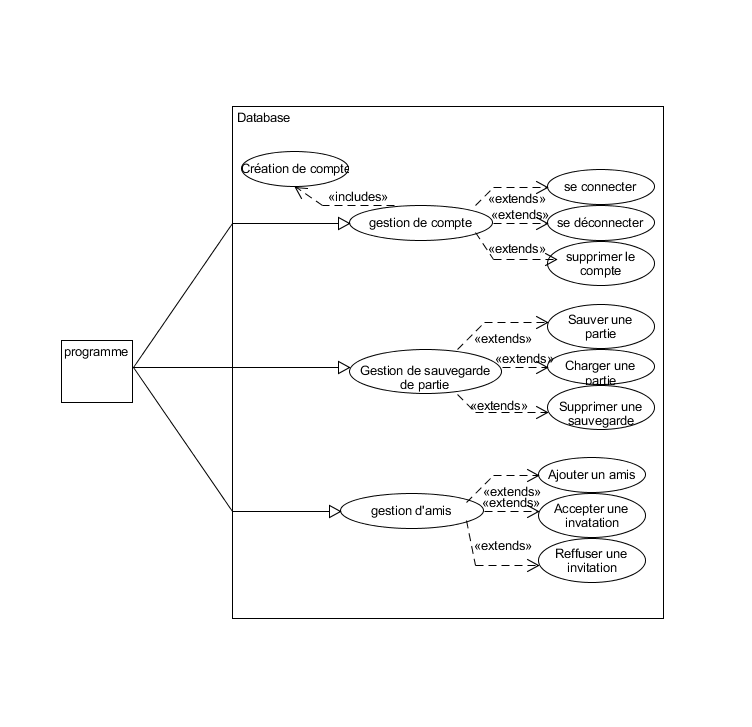
\includegraphics[scale=0.6]{img/DatabaseUseCase.png}
\end{figure}

  \subsection{Gestion des comptes}
    \subsubsection{Création d'un compte}
    \subsubsection{Suppression d'un compte}
  \subsection{Gestions des profils}
    \subsubsection{Affichage des profils}
    \subsubsection{Chat inter-profil}
    \subsubsection{Modifier son profil}
    \subsubsection{Sauvegarder les statistiques du joueur}
  \subsection{Gestion d'une partie}
    \subsubsection{Gestion du plateau}
    \subsubsection{Gestion des pions}
    \subsubsection{Gestion des murs}
    \subsubsection{Gestion des tours}
  \subsection{Rejoindre une partie}
    \subsubsection{Matchmaking rapide: trouver un salon ouvert}
    \subsubsection{Rejoindre un ami}
  \subsection{Classement des joueurs}



\section{Besoins système: Non fonctionnels}
  \subsection{OS}
  \subsection{Réseau}
  \subsection{Disponibilité}
  \subsection{Performances}
  \subsection{Capacité}
  \subsection{Sécurité}
  \subsection{Robustesse}

\newpage
\section{Design et fonctionnement du Système}
  \subsection{Design du système}
  (sans Player)
  \begin{figure}[H]
    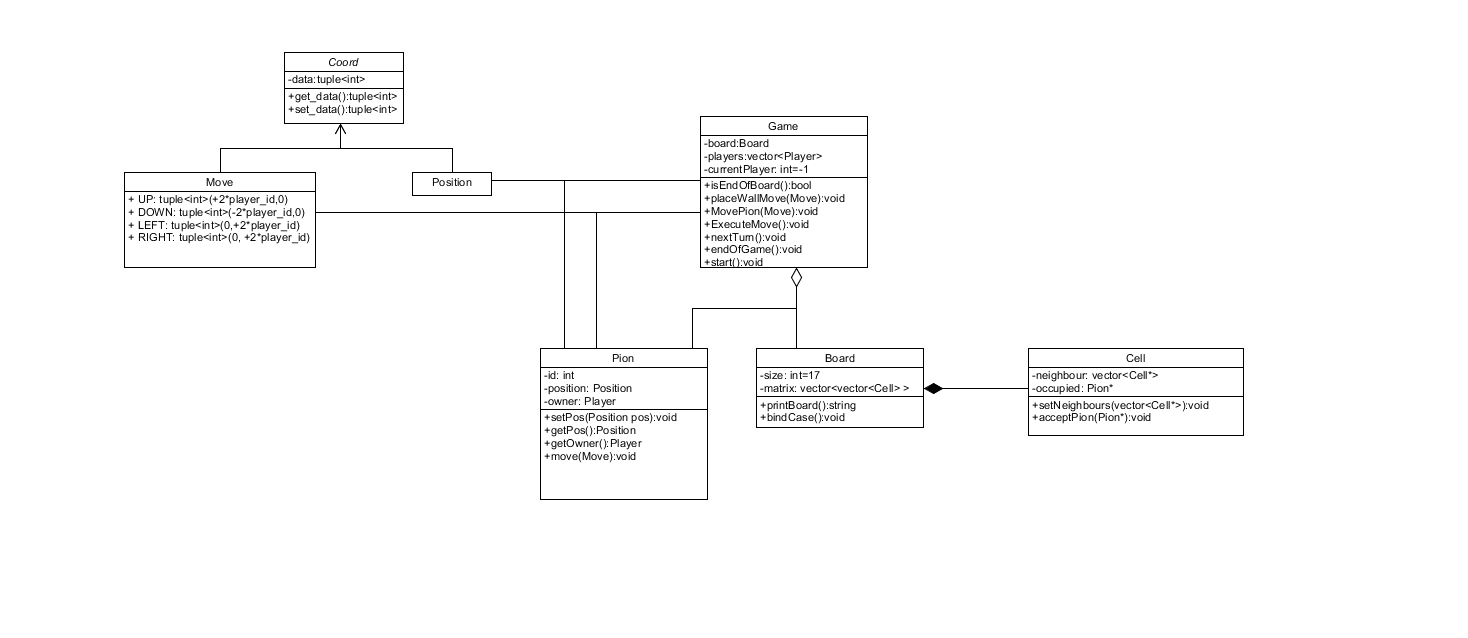
\includegraphics[scale=0.41]{img/MainClassDiagram.png}
  \end{figure}

    \subsubsection{Explications complémentaires}
  \subsection{Fonctionnement du système}
    \subsubsection{Inscription}
    \subsubsection{Connexion}
    \subsubsection{Chat}
  \subsection{Design des modes de jeux}
  \subsection{Design de l'IA}



%------------------------------------------------------------------------------
\end{document}
